\section{Introduction}
Navigation systems have become a popular subject in the designing of unmanned and autonomous systems in recent years. Still, most navigation systems highly depend on the Global Navigation Satellite System (GNSS) receivers as the central resource of navigation data. Although the satellite system can deliver accurate and long-term positioning in open spaces, when relying on GNSS only localization, there are often circumstances when the satellite signal is obstructed or weakened, resulting in degradation or even loss of position estimate precision \cite{ioannides2016known}. Such is especially threatening in high urbanized centers where satellite signals can suffer multipath propagation from tall glass-covered buildings \cite{omar2016integration}. Satellite positioning is especially impactful in battery autonomy, whereas GNSS receivers remain draining a substantial amount of electric current. Inevitably, there is a need to become less dependent on GNSS-based localization, particularly in autonomous settings. Substantial research has been conducted to enhance the localization precision of an object devoid of satellite signals \cite{nassar2004improving}\cite{dewhirst2016improving}\cite{kao1991integration}\cite{coyte2013displacement}\cite{wong1988high}. Increased accuracy is a precursor to establishing autonomous agents for a diversity of functions. Inertial measurement units (IMU) have become standard in embedded inertial systems due to their low cost, lightweight, and low power consumption. They can provide short-term position and orientation changes. Furthermore, inertial systems have been employed in wearable applications with uses in unmanned aerial vehicles (UAV) \cite{hetenyi2016sensor}\cite{luo2013uav}\cite{sharma2014sensor}, telemedicine \cite{madgwick2020extended}, and robotics \cite{wilson2019formulation}. Despite these accomplishments, inertial systems suffer from rapid drift owing to the existence of disturbances and noise in the measurements. Practically all present commercial applications are restricted to minimal motion recognition. Position and orientation in real-world applications are rarely employed due to difficulties in precise integration. Recently, innovative fusion algorithms have emerged, which can diminish the impacts of noise and disturbances, broadening these devices’ capabilities. There is an increasing need, which remains unmet, for inertial orientation and position applications since they are key to automation and the “Internet of Things” (IoT).
We propose a low-cost, multipurpose inertial solution exploring the Internet of Things with modules for an Inertial Measurement Unit that may support maintaining high levels of orientation and location exactness even when satellite-based location is not possible.

\subsection{Problem Statement}
This dissertation explores three core challenges that remain with significant interest in literature.
%satellite-based radio-navigation service is power-hungry, and there is a need for more passive solutions.

\paragraph{A. GNSS only positioning is prone to signal jamming and impacts battery autonomy}
Modern navigation relies greatly on the Global Navigation Satellite System (GNSS) constellations (such as GPS, Galileo, GLONASS, etc.); being straightforward to operate, accurate and trustworthy, it is widely employed in navigation systems. Nevertheless, GNSS signals still encounter numerous vulnerabilities and can often be compromised by natural and human sources~\cite{ioannides2016known}. Attacks against GNSS-based localization are becoming more frequent and of intensifying damage~\cite{papadimitratos2008protection}. Satellite signals can also be affected by abnormal activity due to solar winds, creating temporary gaps in coverage~\cite{amin2016vulnerabilities}.
Moreover, while GNSS offers seamless navigation with inexpensive receivers, they are also prone to signal jamming, where satellites are unable to detect the objects. Repeatedly, position accuracy is reduced or even lost, such as in tunnels or underground sections~\cite{pinker1999vulnerability}~\cite{omar2016integration}. Furthermore, GNSS cannot accurately determine altitude with the necessary exactness, which is essential to accurately depict a body in three-dimensional space.
Lastly, localization technologies demand high processing capacity and communication costs. This is particularly impactful in autonomous settings, where battery autonomy is crucial, while GNSS receivers continue to drain a large amount of electric current~\cite{lo2016greener}. Consequently, power optimization is critical, and there is a necessity to become less reliant on GNSS-based localization.


\paragraph{B. Dead reckoning is susceptible to cumulative errors and suffers from gimbal lock} %Dead reckoning uses Euler angles, trigonometry which makes gimbal lock
When understanding the alternatives to GNSS for estimating the position, the dead reckoning technique is often employed to resolve the location of a moving object. Using sensor data (gyroscope, accelerometer, magnetometer, etc.), it is possible to assess current position even when GNSS positioning is not possible~\cite{omar2016integration}. It has been recognized as a low-power alternative to GNSS localization that can deliver high‐resolution position data~\cite{dewhirst2016improving}. It is possible to estimate the current position from an obtained distance (which may be estimated from velocity), the known starting point, and estimated drift. However, the precision of the dead-reckoning approach is continuously worsening while measurement errors accumulate during the current position estimation~\cite{kao1991integration}. The approach is also embedded in Kalman filtering and other fusion techniques (will be explored in Section II), which mathematically merges a series of navigation solutions to obtain the best estimate of the navigator’s current position, velocity, attitude angles, etc~\cite{krakiwsky1988kalman}.

Still, precise tracking of a moving and rotating body in three-dimensional space implies a superior degree of complexity (compared to two-dimensional tracking). It can be accomplished in a range of approaches. Most commonly, the orientation of bodies that move in three dimensions may be explained by a combination of their angle of rotation across each of their three axes (e.g., such as in trigonometry, where Euler angles can approximate yaw, roll, and pitch). Fundamentally, a specific movement could be defined by multiple rotations. In such case, to perform a rotation over a particular axis, rotational matrices, vector operations, and trigonometric functions are required~\cite{bojanczyk1991computation}. This involves numerous complex mathematical operations and several clock cycles in a microprocessor that could negatively impact computational performance~\cite{janota2015improving}.

Nevertheless, the rotation axes are not always independent, and results are not necessarily distinctive or unique. This further implies that the plane of two gimbals (rotational axes) to align, which causes the recognized gimbal lock phenomenon, where two out of three gimbals are parallel or very nearly parallel (such as in figure \ref{fig:gimballock}.b), reducing the output to two degrees of freedom \cite{hemingway2018perspectives}. When gimbal lock happens, it is not possible to reorientate the axes without an external reference.
% Alternatives using quaternions may be used, while most studies apply them in microcomputers rather than on microcontrollers. Quaternions give the capability to define any three-dimensional rotation around an axis distinctively and are not susceptible to gimbal lock \cite{alaimo2013comparison}.

\begin{figure}[!h]
      \centering
      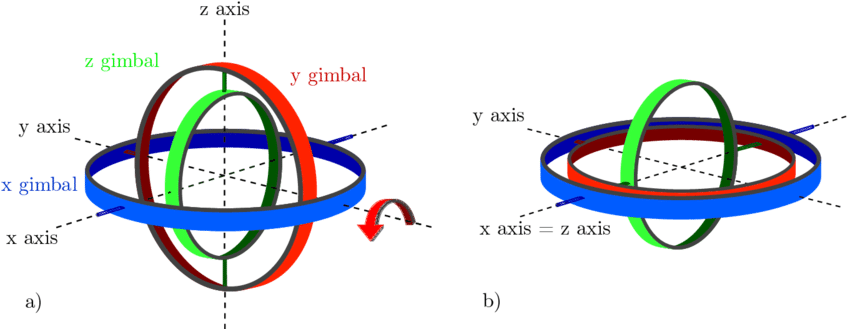
\includegraphics[width=0.7\textwidth]{figures/gimbal_lock.png}
      \caption{Representation of the Gimbal Lock problematic \cite{zeitlhofler2019nominal} - The exterior blue gimbal characterizes the x-axis, the middle, red-colored gimbal the y axis, and the inner green gimbal the z-axis. In the initial arrangement a), every axis is perpendicular to one another. Following a rotation of 90º across the red arrow (y-axis), the blue and the green gimbals occupy the same rotation axis. This condition inhibits the clear determination of the rotation axes when subsequently rotating around the x or z-axis. }
      \label{fig:gimballock}
\end{figure}

\paragraph{C. Gravity acceleration greatly impacts sensor readings}
An accelerometer is generally utilized to estimate the velocity and position of a given body devoid of the usage of GNSS. These electromechanical devices can measure proper acceleration forces, which can be employed to determine a body’s velocity and position relative to a starting point. In theory, this can be done by integrating the resultant of acceleration yielding velocity; double integrating will deliver the body’s accumulative position~\cite{yang2006simple}. In practice, these measurements are influenced by Earth’s gravitational field and rotational components of acceleration, significantly magnifying numerical errors during the readings~\cite{nistler2011gravity}. The gravity component will not be differentiated from the physical acceleration of the device and will eventually generate exceedingly elevated errors in the measured acceleration. Double integrating these measurements will inherently amplify errors which will accumulate exponentially, translating into a yet greater offset in velocity and position estimates~\cite{thong2004numerical}.

A potential solution to minimize this difficulty is to assume the body moves on a flat surface, thus greatly diminishing the influence of the gravity component on acceleration readings. Every inaccuracy that may arise from hiring such supposition can be regarded as noise and is smoothly filtered~\cite{nistler2011gravity}. Understandably, such an assumption is not possible with a body moving through three-dimensional space since it is subject to many kinds of forces and movements.  A numerical process is required for handling accelerometer measurements that utterly removes the effect of the gravity component and further undesirable acceleration vectors.




% Dead Reckoning
% Euler angles
% Estimation using Trigonometry
% Sensor data (IMU)
% AHRS  - Attitude Heading Reference System
% Pitch, Roll, and Yaw
% Complementary filters
% Kalman filters
% inertial measurement unit (IMU) sensing packages are revolutionizing mature industries, “turning agriculture into smart agriculture, infrastructure into Smart infrastructure, and cities into Smart cities,” - https://ieeexplore.ieee.org/document/9103115


\subsection{Research Questions}
While research has been performed towards orientation estimation by the fusion of multiple sensors, few studies sought to assess position due to difficulties removing the measurement of normal forces that do not cause physical acceleration of the sensor. This investigation seeks to comprehend how different sensor fusion approaches perform in approximating the orientation of a moving system, along with how to overcome the positioning challenge through a technique that combines orientation estimation to filter non-physical acceleration. Additionally, we examine how the Internet of Things can be applied to perform telemetry in real-time and at a long distance of a moving object.

\begin{itemize}
      \item \textbf{[RQ1]. Estimate} - How to perform a low-cost orientation and position estimation of a moving object devoid of GNSS?\\
            The study will emphasize on the possibility of estimating the orientation and position of a moving object in three-dimensional space short of GNSS-based positioning by combining multiple low-cost sensors to provide an object’s navigation information.
      \item \textbf{[RQ2]. Comparing} - How distinct fusion techniques perform in orientation and position estimation? \\
            An experimental comparison between various sensor fusion algorithms is used to evaluate how accurate each approach can approximate orientation and position.
      \item \textbf{[RQ3]. Communicate} - How to transmit navigational data in real-time at a long-distance?\\
            Lastly, this dissertation will explore the prospect of amalgamating transmission IoT devices (based on open radio frequency at 868 MHz) to broadcast in real-time and at a long distance the navigational data of a moving object and how this approach may be employed in a series of real-world scenarios.

\end{itemize}